%-------------------------------------------------------%
\section{初期値/境界値データの作成:init} \label{sec:tutorial_real_init}
%-------------------------------------------------------%

\verb|init|ディレクトリに移動し、\scalerm によるシミュレーションに必要な初期値/境界値データを作成する。
\begin{verbatim}
 $ cd ${Tutorial_DIR}/real/experiment/init
 $ ls
    Makefile
    init.d01.conf
    init.launch.conf
    param.bucket.conf
    scale-rm_init
\end{verbatim}
ディレクトリの中には、設定ファイル\verb|init.d01.conf|が準備されている。
他に\verb|init.launch.conf|というファイルも存在するが、ここでは使用しない。
\verb|init.d01.conf|ファイルには表\ref{tab:grids}に示すチュートリアル用の設定が
既になされているが、\verb|pp.d01.conf|と同様に実験設定に応じて変更されたい。
初期値/境界値データの生成には、前節で作成した地形データが使用される。
地形データは、\verb|init.d01.conf|において相対パスで設定する。

\editbox{
\verb|&PARAM_TOPOGRAPHY| \\
\verb|   TOPOGRAPHY_IN_BASENAME = "../pp/topo_d01",| \\
\verb|/| \\
 \\
\verb|&PARAM_LANDUSE| \\
\verb|   LANDUSE_IN_BASENAME = "../pp/landuse_d01",| \\
\verb|/| \\
}
その他に、\verb|init.d01.conf|の設定の中で特に確認して欲しい項目は、
\namelist{PARAM_MKINIT_REAL_ATMOS}、
\namelist{PARAM_MKINIT_REAL_OCEAN}、
\namelist{PARAM_MKINIT_REAL_LAND}の項目である。

\editboxtwo{
\verb|&PARAM_MKINIT_REAL_ATMOS| & \\
\verb| NUMBER_OF_FILES      = 2,|                                   & {\small ← 読み込むファイルの数} \\
\verb| FILETYPE_ORG         = "GrADS",|                             & {\small ← 表\ref{tab:inputdata_format}から選択する} \\
\verb| BASENAME_ORG         = "namelist.grads_boundary.FNL.2005053112-2015011400",| & \\
\verb| BASENAME_BOUNDARY    = "boundary_d01",|                      & {\small ← 境界値データの出力名} \\
\verb| BOUNDARY_UPDATE_DT   = 21600.0,|                             & {\small ← 入力データの時間間隔} \\
\verb| PARENT_MP_TYPE       = 3,|                                   & \\
\verb| USE_FILE_DENSITY     = .false.,|                             & {\small ← 親モデルの大気密度データを使うか} \\
\verb|/| \\
\\
\verb|&PARAM_MKINIT_REAL_OCEAN| & \\
\verb|   ..... 略 .....              |  & \\
\verb| INTRP_OCEAN_SFC_TEMP = "mask",|                              & {\small ← SSTの欠測値処理方法} \\
\verb| INTRP_OCEAN_TEMP     = "mask",|                              & {\small ← SSTの欠測値処理方法} \\
\verb|/| \\
\\
\verb|&PARAM_MKINIT_REAL_LAND| & \\
\verb|   ..... 略 .....              | & \\
\verb| USE_FILE_LANDWATER   = .true.,|                              & {\small ← 親モデルの土壌水分データを使うか} \\
\verb| INTRP_LAND_TEMP      = "mask",|                              & {\small ← 土壌温度の欠測値処理方法} \\
\verb| INTRP_LAND_WATER     = "fill",|                              & {\small ← 土壌水分の欠測値処理方法} \\
\verb| INTRP_LAND_SFC_TEMP  = "fill",|                              & {\small ← 地表面温度の欠測値処理方法} \\
\verb|/| \\
}

気象場データのファイル形式は\nmitem{FILETYPE_ORG}で指定する。
ここでは、{\grads}形式のデータを読み込むために``\verb|grads|''を与えている。
入力ファイルの詳細は第\ref{sec:adv_datainput}節を参照されたい。

第\ref{sec:tutorial_real_data}節でバイナリ形式に変換した入力データ(FNL)へのリンクを、
作業ディレクトリに張る。リンクを適切に張るために、\verb|${Tutorial_DIR}/real/data|の中に「\verb|gradsinput-link_FNL.sh|」というスクリプトを用意している。
\begin{verbatim}
  $ cp ../../data/gradsinput-link_FNL.sh ./
  $ sh gradsinput-link_FNL.sh
\end{verbatim}
上記のコマンドを実行し、下記のリンクが作成されていれば成功である。
\msgbox{
\verb|ATM_00000.grd -> ../tools/FNL_output/200707/FNL_ATM_2007071418.grd| \\
\verb|ATM_00001.grd -> ../tools/FNL_output/200707/FNL_ATM_2007071500.grd| \\
\verb|LND_00000.grd -> ../tools/FNL_output/200707/FNL_LND_2007071418.grd| \\
\verb|LND_00001.grd -> ../tools/FNL_output/200707/FNL_LND_2007071500.grd| \\
\verb|SFC_00000.grd -> ../tools/FNL_output/200707/FNL_SFC_2007071418.grd| \\
\verb|SFC_00001.grd -> ../tools/FNL_output/200707/FNL_SFC_2007071500.grd| \\
}

次に、{\grads}形式のバイナリデータを{\scalelib}で読み込むためのネームリストファイルを、
ディレクトリ\verb|init|へリンクする。
\begin{verbatim}
  $ ln -s ../../data/namelist.grads_boundary.FNL.2005053112-2015011400 ./
\end{verbatim}
%
上記の準備が完了したら、4つのMPIプロセスを使用して\verb|scale-rm_init|を実行する。
\begin{verbatim}
 $ mpirun -n 4 ./scale-rm_init init.d01.conf
\end{verbatim}

正常にジョブが終了すれば、以下のファイルが生成される。
\begin{verbatim}
 $ ls
    boundary_d01.pe000000.nc
    boundary_d01.pe000001.nc
    boundary_d01.pe000002.nc
    boundary_d01.pe000003.nc
    init_d01_20070714-180000.000.pe000000.nc
    init_d01_20070714-180000.000.pe000001.nc
    init_d01_20070714-180000.000.pe000002.nc
    init_d01_20070714-180000.000.pe000003.nc
    init_LOG_d01.pe000000
\end{verbatim}
\verb|init_LOG_d01.pe000000|はログファイルであり、
処理が正常に完了していれば、ファイルの最後に
\msgbox{
 +++++ Closing LOG file\\
}
が出力される。
\verb|boundary_d01.pe######.nc|は境界値データ、
\verb|init_d01_20070714-180000.000.pe######.nc|は初期値データであり、
各ファイルのサイズは約18.9 MB、約12.6 MB である。
ここで、\verb|######|はMPIプロセス番号を表す。\\

\vspace{0.8cm}
\noindent {\Large\em NOTICE}: {\large 入力データ読み込み時のメモリ節約} \hrulefill

\scalerm では、初期値データの読込はマスタープロセスのみが行い、broadcast通信によって各ノードに情報を伝播する。
これはできるだけファイルIOを減らし、高速に初期値データを処理するためのアルゴリズムである。
一方でこのアルゴリズムは、特に大規模並列計算システムにおいて、大きな初期値データを読み込む際に、メモリ容量が足りなくなることがある。
これを回避するために、下記のように、各ノードが自身に必要なデータだけを読み込む方式に切り替えることで、メモリ不足を解消することができる。
%
\editboxtwo{
\verb|&PARAM_MKINIT_REAL_ATMOS| & \\
\verb| SERIAL_PROC_READ = .false.,| & {\small ← マスタープロセスのみデータにアクセスするかどうか} \\
\verb|/| \\
}
デフォルト設定は\verb|.true.|であり、マスタープロセスのみファイルIOを実行する。
\verb|.false.|にすると、各ノードがファイルIOを行うことで使用するメモリ量を削減する。
ただしファイルIOが増大するため、システムによってはファイルアクセスをロックされる等、パフォーマンスの低下がありうることに注意。

\noindent \hrulefill\\


\vspace{0.8cm}
\noindent {\Large\em OPTION} \hrulefill \\
「gpview」がインストールされている場合は、以下のコマンドによって
初期値と境界値が正しく作成されているかを確認できる。

\begin{verbatim}
 $ gpvect --wsn=1 --scalar --slice z=1500 --nocont --aspect=1 --range=0.002:0.016         \
          --int 0.001 --xintv=10 --yintv=10 --unit_vect                                   \
          init_d01_20070714-180000.000.pe00*@QV  init_d01_20070714-180000.000.pe00*@MOMX  \
          init_d01_20070714-180000.000.pe00*@MOMY --title "QV, MOMX, MOMY"
\end{verbatim}
処理が正常に終了していれば、図\ref{fig:init}と同様の図が得られる。

\begin{figure}[h]
\begin{center}
  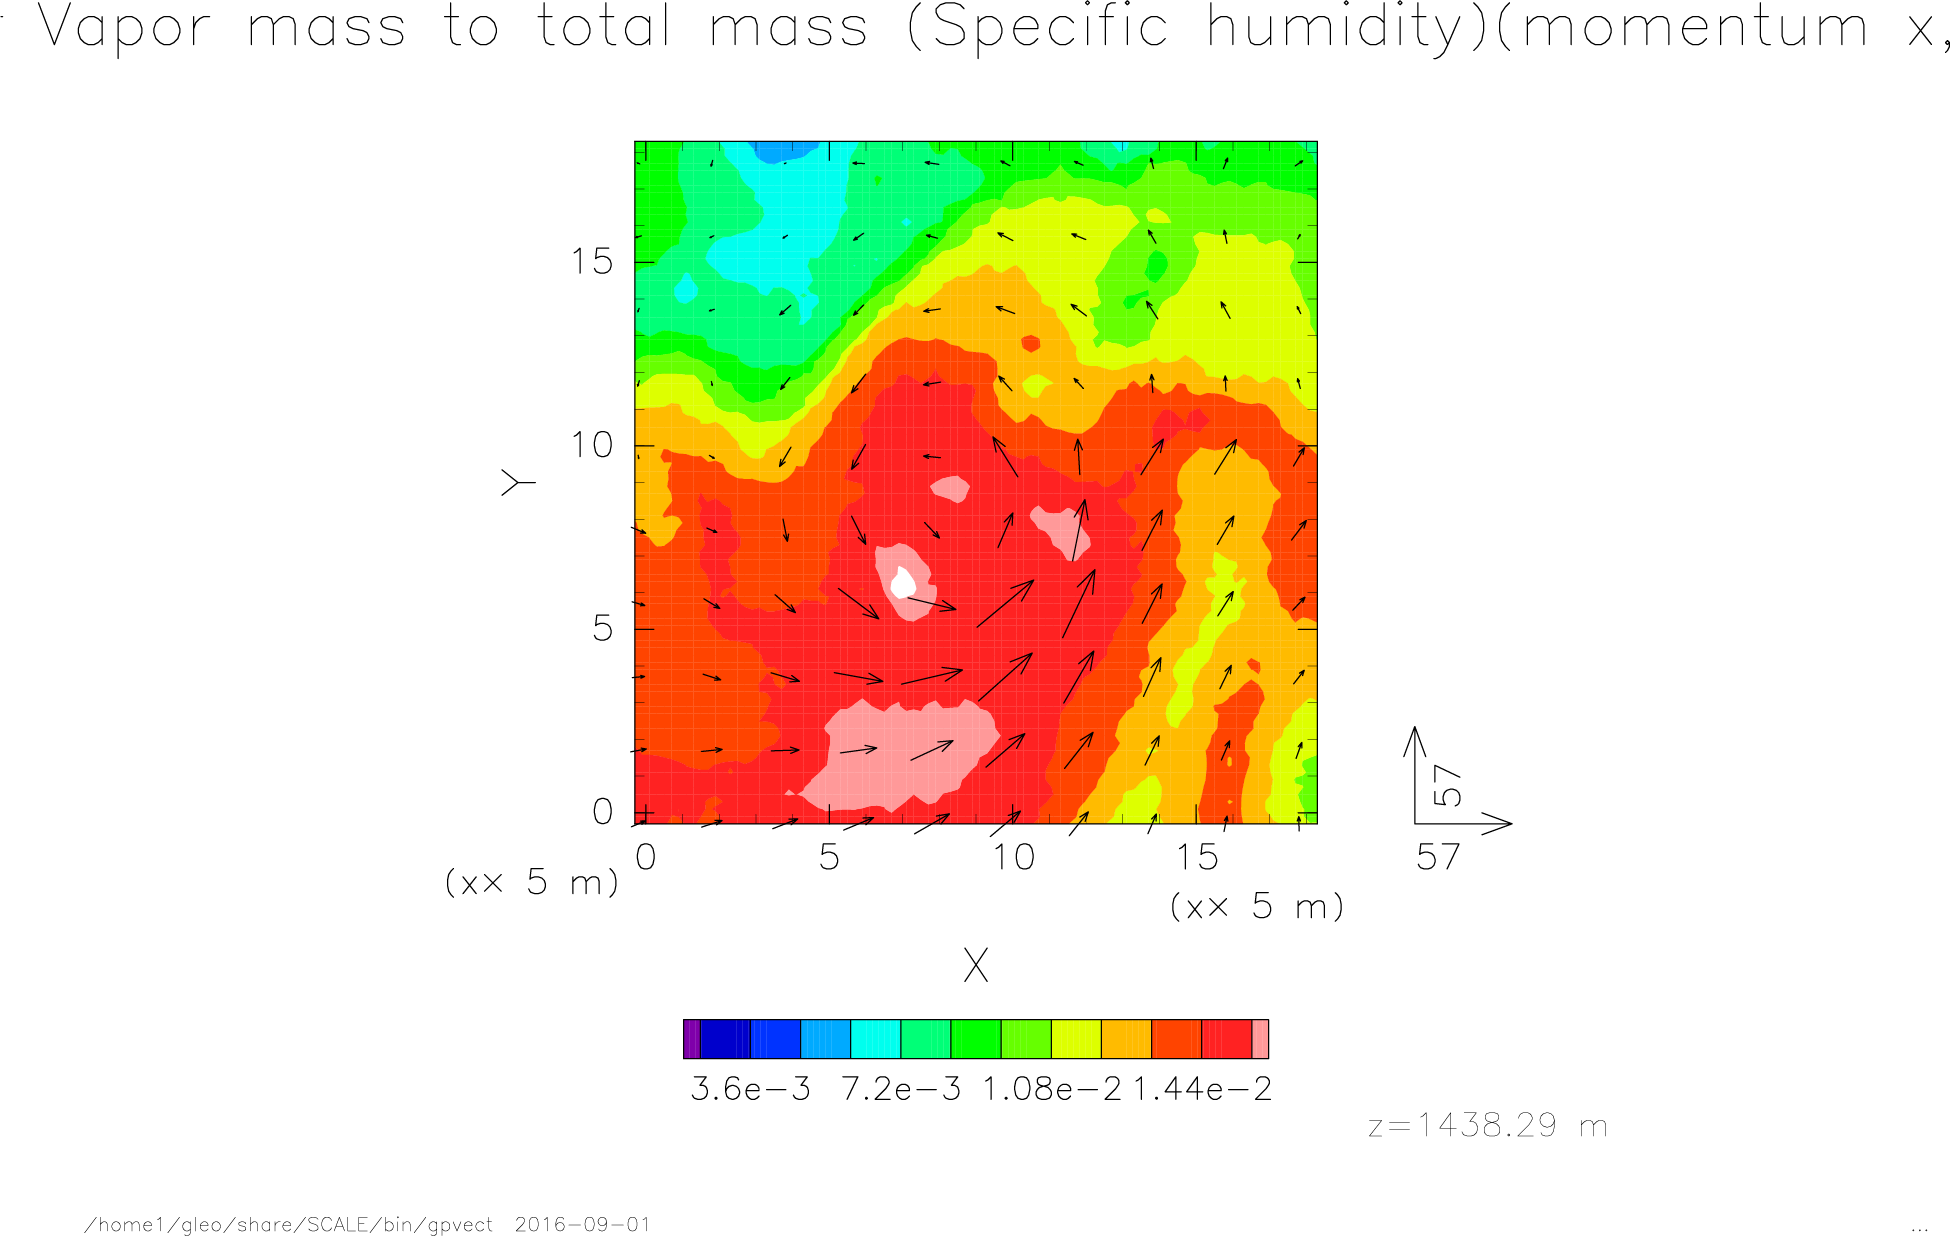
\includegraphics[width=0.9\hsize]{./../../figure/real_init_qv-momxy.pdf}\\
  \caption{チュートリアル実験における初期場の様子($z=$1500 m)。
           色は比湿、ベクトルは水平運動量フラックスを表す。}
  \label{fig:init}
\end{center}
\end{figure}
